%%%% fatec-article.tex, 2024/03/10

%% Classe de documento
\documentclass[
  a4paper,%% Tamanho de papel: a4paper, letterpaper (^), etc.
  12pt,%% Tamanho de fonte: 10pt (^), 11pt, 12pt, etc.
  english,%% Idioma secundário (penúltimo) (>)
  brazilian,%% Idioma primário (último) (>)
]{article}

%% Pacotes utilizados
\usepackage[]{fatec-article}
\Author{1}{Name={Autor 1\\ Autor 2 \\ Autor 3\\ Autor 4}}

\Author{2}{Name={\{ autor1@fatec.sp.gov.br \}\\ \{ autor2@fatec.sp.gov.br \} \\ \{ autor3@fatec.sp.gov.br\} \\ \{ autor4@fatec.sp.gov.br \}}}

%% Definição das palavras-chaves/keywords
\Keyword{1}{Artigo}{Article}
\Keyword{2}{Latex}{Latex}
\Keyword{3}{Informática}{Informatic}

%%%% Resumo no idioma primário (brazilian)
\begin{Abstract}[brazilian]%% Idioma (brazilian ou english)
  O resumo FATEC Registro é uma descrição completa e concisa dos componentes-chave da metodologia do estudo e dos achados importantes da pesquisa. Normalmente, o resumo é o primeiro encontro do leitor com uma pesquisa ou relato, sendo algumas vezes o único elemento recuperado e/ou revisado nas bases de dados científicos. Esse elemento provê a primeira impressão, muitas vezes a mais importante, identificando o valor potencial ou a relevância do enfoque da pesquisa e dos resultados. Se o resumo for bem escrito, ele atrairá leitores para obter uma cópia do manuscrito completo que será incorporado aos que já foram encontrados, e seu trabalho será citado. Se o resumo for mal escrito, a pesquisa poderá ser ignorada ou, até mesmo, esquecida.
\end{Abstract}

%%%% Resumo no idioma secundário (english)
\begin{Abstract}[english]%% Idioma (brazilian ou english)
The summary is a complete and concise description of the key components of the study methodology and important research findings. Typically, the summary is the reader's first encounter with a research report or paper, and sometimes it is the only element retrieved and/or reviewed in scientific databases. This element provides the first impression, often the most important one, identifying the potential value or relevance of the research approach and findings. If the summary is well-written, it will attract readers to obtain a copy of the full manuscript that will be incorporated into those already found, and your work will be cited. If the summary is poorly written, the research may be ignored or even forgotten.
\end{Abstract}

%% Processamento de entradas (itens) do índice remissivo (makeindex)
\makeindex%

%% Arquivo(s) de referências
\addbibresource{fatec-article.bib}

%% Início do documento
\begin{document}

% Seções e subseções
%\section{Título de Seção Primária}%

%\subsection{Título de Seção Secundária}%

%\subsubsection{Título de Seção Terciária}%

%\paragraph{Título de seção quaternária}%

%\subparagraph{Título de seção quinária}%

\section*{Introdução}%
\label{sect:intro}
Uma boa introdução precisa informar ao leitor de forma clara e objetiva o que será trabalhado no desenvolvimento e na conclusão do texto. Nela, apresentam-se os principais temas que serão discutidos ao longo do conteúdo, então deve servir como um convite para que o texto seja lido até o final.

A introdução é essencial para motivar o público a conferir o conteúdo por inteiro. Além desse convite decisivo, é nela que o objetivo do texto deve ser destacado: (1) Porque o artigo é relevante? e (2) Como ele pode contribuir para a vida do leitor?.





\section*{OBJETIVO} \label{sect:obj}

a) Desenvolver um algoritmo de PLN capaz de analisar o conteúdo textual de páginas da \textit{Web} e identificar padrões linguísticos associados a conteúdos discriminatórios, injuriosos ou que incitem discurso de ódio.

b) Integrar o sistema de auditoria de conteúdo \textit{Web} com um sistema de notificação, de forma que o usuário seja alertado na tela quando for identificado conteúdo ofensivo ou prejudicial, incluindo informações sobre o motivo do bloqueio e opções para revisão por administradores escolares, caso necessário.

c) Funcionalidade de retroalimentação, permitindo que o sistema aprenda continuamente com novos dados, aprimorando sua capacidade de identificação e bloqueio de conteúdos prejudiciais através do feedback dos administradores ou de atualizações periódicas de dados e padrões linguísticos.

d) Desenvolver um painel de controle administrativo, que permita a visualização de estatísticas sobre tentativas de acesso bloqueadas, tipos de conteúdo identificado, e histórico de notificações, oferecendo também a possibilidade de personalizar critérios de bloqueio de acordo com as políticas da instituição.

\section*{ESTADO DA ARTE} \label{sect:estadoarte}

Nesta seção, você deverá realizar um mapeamento de toda a produção acadêmica sobre o tema do seu projeto. É um processo bastante importante porque reúnem todas as pesquisas e descrevem as conclusões das pesquisas sobre o tema \cite{smith:99}. Para escrever um bom estado da arte, você poderá utilizar algumas perguntas norteadoras, tais como:

\begin{enumerate}
    \item O que as atuais pesquisas científicas concluíram sobre o tema?
    \item Quais as divergências dos pesquisadores sobre o assunto?
    \item Quem está pesquisando sobre esse tema?
    \item Onde estão fazendo essas pesquisas?
\end{enumerate}

Em outras palavras, o estado da arte destaca os aspectos de outras pesquisas, mas também identifica as lacunas que existem nessas pesquisas. Ou seja: analisa o que as pesquisas falaram e o que não falaram sobre o tema \cite{Alencar2007,Beltrano2021,Fulano2021}.

Segundo \textcite{Ramos2003,Carvalho2004}, para que você possa descrever as pesquisas/trabalhos que estão relacionados ao seu, não esqueça de citá-los ao decorrer do texto. Para isso, você poderá utilizar o comando $\backslash$cite para citação implícita ou o comando $\backslash$textcite para citações explícitas.

As citações diretas curtas (de até três linhas) acompanham o corpo do texto e se destacam com aspas duplas. Caso o texto original já contenha aspas, estas devem ser substituídas por aspas simples. Enquanto que, para representar as citações diretas longas (com mais de três linhas), estas devem ser transcritas em parágrafo distinto, da seguinte forma:

\begin{displayquote}
   Toda citação direta com mais de três linhas é considerada uma citação direta longa.
Este tipo de citação deve ser escrita sem aspas, em parágrafo distinto, com fonte de tamanho 10, espaçamento simples e com recuo de 4cm da margem esquerda, terminando na margem direita, conforme ilustrado neste exemplo \cite{Andujar2006}.
\end{displayquote}

Vale ressaltar que a utilização de citações diretas longas deve ser evitada durante a escrita de artigos científicos. Conforme visto em \textcite{Kalakota2002,Purcidonio2008}, os dados de cada referência podem ser obtidos de um arquivo com a extensão bib, geralmente na própria página de \textit{download} da referência (artigos, livros, etc.) ou, ainda, a partir do Google Acadêmico, etc.



\section*{METODOLOGIA} \label{sect:metodologia}

A seção de Metodologia explica aos leitores quais procedimentos, abordagens, desenhos e tratamento realizamos na pesquisa, o que permitirá replicar os estudos, entender a linearidade entre a abordagem dos objetivos e os resultados obtidos, determinar sua adequação e relevância e evidenciar qualquer viés na maneira como o estudo foi elaborado e realizado. Em outras palavras, é uma estrutura contextual que apresenta um caminho lógico para responder a perguntas que você levanta no início de sua tese ou artigo \cite{knuth:84}. 

É importante que nesta seção, você descreva todas as ferramentas e tecnologias utilizadas para o desenvolvimento da sua pesquisa \cite{boulic:91}. Lembre-se de detalhar para que serve cada ferramenta e tecnologia e o motivo da sua escolha.


\section*{RESULTADOS PRELIMINARES}\label{sect:resultados}

O propósito da seção de resultados, como o próprio nome indica, é revelar o que foi encontrado na pesquisa. Essa parte do artigo estará composta dos dados relevantes obtidos e sintetizados pelo autor. 

Nesta seção, você deverá apresentar todos os elementos solicitados no mapa mental relacionados ao seu projeto: diagramas, protótipos, modelo de negócios, principais funções e componentes desenvolvidos. Para tanto, na subseção a seguir, você poderá consultar como é feita a inserção de figuras, fluxogramas, fotografias, gráficos, tabelas e quadros.

\subsection*{Ilustração e Tabela}

Independentemente da ilustração (figura, fluxograma, fotografia, gráfico, quadro, entre outras) ou tabela inserida no trabalho, sua identificação deve aparecer na parte superior. Esta identificação deve ser precedida da palavra designativa, seguida de seu número de ordem de ocorrência no texto, em algarismos arábicos, travessão e do respectivo título.

Após a ilustração ou tabela, na parte inferior, indicar a fonte consultada (mesmo sendo produção do próprio autor), legenda, notas e outras informações necessárias à sua compreensão (se houver). A ilustração deve ser citada no texto e inserida o mais próximo possível do trecho a que se refere. A seguir, encontra-se um exemplo para a inserção de um elemento do tipo Gráfico, o \Cref{grph:example}.

\begin{graph}[!h]
\centering
\SetCaptionWidth{\ifbool{@LayoutA}{0.7}{0.72}\linewidth}
\caption{Exemplo de gráfico}%
\label{grph:example}
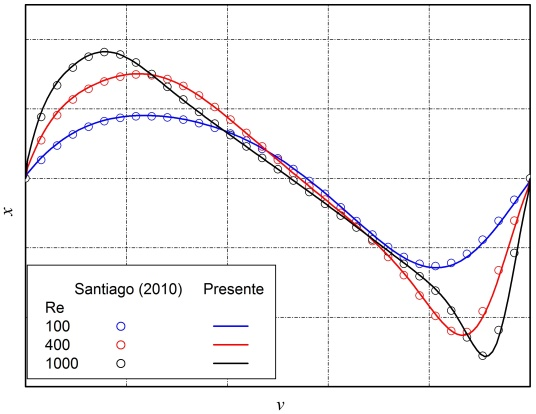
\includegraphics[width = \CaptionWidth]{grph-example}
\SourceOrNote{Autoria Própria (2024)}
\end{graph}

Em computação, é muito comum a utilização de fluxogramas, para documentar, estudar, planejar, melhorar e comunicar processos complexos por meio de diagramas claros e fáceis de entender. Um fluxograma é um diagrama que descreve um processo, sistema ou algoritmo de computador. O \Cref{fcht:ex-algorithm} é um dos vários exemplos deste tipo de ilustração que pode ser gerado ou editado na ferramenta \textit{online} \href{http://www.lucidchart.com/}{Lucidchart}, entre outras.

\begin{flowchart}[!htb]
\centering
\caption{Exemplo de fluxograma de algoritmo}%
\label{fcht:ex-algorithm}
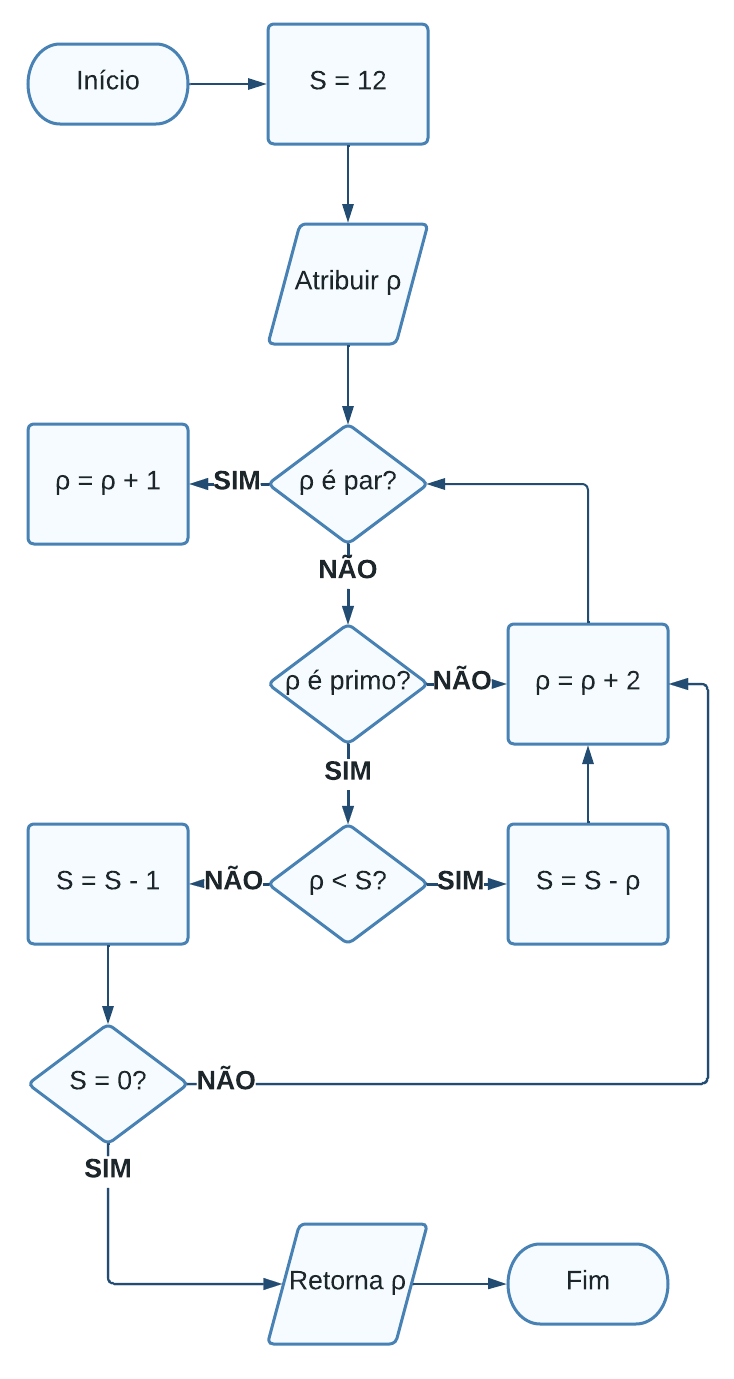
\includegraphics[scale=0.4]{fcht-ex-algorithm}
\SourceOrNote{Autoria Própria (2024)}
\end{flowchart}

O LaTeX tem uma biblioteca específica para utilizar imagens no documento. O pacote graphicx habilita um ambiente chamado figure, que permite que você insira imagens de uma forma simples no texto. A \Cref{fig:example-image-duck} é um exemplo deste tipo de ilustração.

\begin{figure}[!h]
\centering
\caption{Exemplo de figura}%
\label{fig:example-image-duck}
\includegraphics[scale=1.2]{example-image-duck}
\SourceOrNote{Autoria Própria (2024)}
\end{figure}

Caso seja necessário, você ainda poderá inserir fotografias, por meio do ambiente \textit{photograph}, conforme ilustrado na \Cref{phot:pg-campus}.

\begin{photograph}[!h]
\centering
\SetCaptionWidth{\ifbool{@LayoutA}{0.7}{0.72}\linewidth}
\caption{Fachada da Fatec de Registro}%
\label{phot:pg-campus}
\savebox0{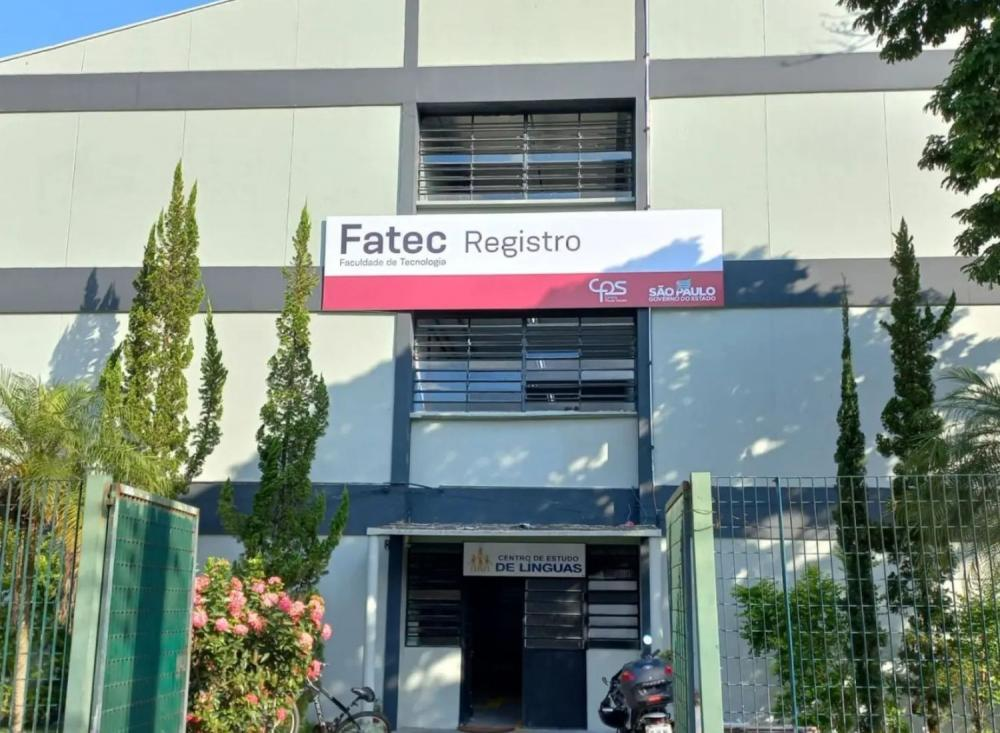
\includegraphics[width = \CaptionWidth]{Illustrations/fachada-fatec.jpg}}
\usebox0%
\SourceOrNote{Autoria Própria (2024)}
\end{photograph}

Outro elemento visual bastante utilizado na seção de Resultados são as tabelas, pois elas fornecem uma estrutura visualmente organizada para apresentar dados, tornando a leitura e a compreensão do conteúdo mais fácil para o leitor. As células, linhas e colunas ajudam a alinhar informações de maneira sistemática.

Para conjuntos de dados comparativos, as tabelas são particularmente úteis. Elas possibilitam a disposição lado a lado de informações relacionadas, facilitando a comparação direta entre diferentes elementos.

Tabelas e quadros devem estar centralizados e conter apenas dados imprescindíveis, evitando-se que sejam muito extensos, não repetindo dados já inseridos no texto, ou vice-versa. O formato de tabela pode ser observado na \Cref{tab:example}.

\begin{table}[!htb]
\centering
\SetCaptionWidth{0.5\linewidth}
\caption{Exemplo de tabela}%
\label{tab:example}
\begin{tabularx}{\CaptionWidth}{@{}XY@{}}
\toprule%
\rowcolor{TableColor}
\multicolumn{1}{Y}{\textcolor{white}{Idade}}           &
\multicolumn{1}{Y}{\textcolor{white}{Percentual (\%)}} \\
\midrule%
Até 20 anos     & 0  \\
De 21 a 30 anos & 10 \\
De 31 a 40 anos & 20 \\
De 41 a 50 anos & 30 \\
\bottomrule%
\end{tabularx}
\SourceOrNote{Adaptada de \textcite{Beltrano2021}}
\end{table}

No caso de quadros, deve ser seguida a estrutura demonstrada no \Cref{tfrm:typography}.
Caso os dados sejam inéditos e provenientes de uma pesquisa realizada pelos próprios autores do trabalho, essa especificação deve constar na fonte com o ano da pesquisa de campo.
Nesse caso, a fonte deve ser: Autoria Própria (2024).

\begin{tabframed}[!htb]
\centering
\caption{Tipografia das seções}%
\label{tfrm:typography}
\begin{tabularx}{\linewidth}{?{}p{20mm}|X|p{45mm}?{}}%% CHKTEX 44
\toprule%
\rowcolor{TableColor}
\multicolumn{1}{?{}c|}{\textcolor{white}{Seção}}   &
\multicolumn{1}{c|}{\textcolor{white}{Tipografia}} &
\multicolumn{1}{c?{}}{\textcolor{white}{Exemplo}}  \\
\midrule%
Primária                     &
Letras maiúsculas em negrito &
\textbf{1 SEÇÃO PRIMÁRIA}    \\
\midrule%
Secundária                    &
Letras maiúsculas sem negrito &
1.1 SEÇÃO SECUNDÁRIA          \\
\midrule%
Terciária                                                             &
Letra inicial de todas as palavras em maiúscula, sem negrito &
1.1.1 Seção Terciária                                                 \\
\midrule%
Quaternária                                                          &
Letra inicial da primeira palavra em maiúscula, sem negrito &
1.1.1.1 Seção quaternária                                            \\
\midrule%
Quinária                                                                          &
Letra inicial da primeira palavra em maiúscula, sem negrito e em itálico &
\textit{1.1.1.1.1 Seção quinária}                                                 \\
\bottomrule%
\end{tabularx}
\SourceOrNote{Autoria Própria (2024)}
\end{tabframed}

Quadros e tabelas podem ser inseridos neste documento usando os ambientes \texttt{tabframed} e \texttt{table}, respectivamente, conforme exemplos no arquivo-fonte deste modelo. A geração ou edição desses elementos visuais pode ser realizada por meio de ferramentas \textit{online}, tais como: \href{http://www.tablesgenerator.com/}{Tables Generator} e \href{http://www.latex-tables.com/}{Latex Tables Editor}, entre outras.

\subsection*{Equações}

Equações podem ser inseridas neste documento usando o ambiente  \texttt{equation}, como ilustrado na \Cref{eq:u}.

\begin{equation}%
\label{eq:u}
u = \beta \operatorname{sen} \left(\pi x\right) \frac{\left(e^{2x} - 1\right) \left(e^y - 1\right)}{\left(e^2 - 1\right) \left(e - 1\right)}
\end{equation}

Símbolos matemáticos (ou equações mais simples) podem ser inseridos ao longo do texto de um parágrafo usando o ambiente do Latex \texttt{math}. É possível ainda, a utilização de ferramentas onlines para a geração ou edição de equações, tais como: \href{http://formulasheet.com/}{Formula Sheet} e \href{http://www.tutorialspoint.com/latex_equation_editor.htm}{Latex Equation Editor}.



\section*{CONCLUSÃO}\label{sect:conclusao}

% Apresente aqui as conclusões do seu trabalho, verifique se o objetivo foi cumprido, apresenta respostas para o problema da pesquisa, relate as limitações e as recomendações do estudo. Por fim, coloque sugestões para trabalhos futuros.
Este artigo destacou a aplicação da tecnologia e da Inteligência Artificial no contexto escolar, com foco na detecção e no bloqueio de acesso a sites com conteúdos discriminatórios. Diante dos crescentes desafios relacionados à inclusão étnica, educacional e social, a adoção de abordagens inovadoras se torna imprescindível para atender às demandas em constante evolução. 

O projeto Resist está alinhado aos Objetivos de Desenvolvimento Sustentável (ODS) da ONU, especificamente ao objetivo quatro, que visa garantir educação inclusiva, equitativa e de qualidade, e ao objetivo dez, que promove a inclusão social, econômica e política, independentemente de características como idade, sexo, raça, etnia, origem, religião ou condição econômica. A implementação do sistema transcende a simples detecção de conteúdos discriminatórios, abrangendo também o bloqueio de sites que contenham contextos de intolerância. Além disso, possibilita que instituições de ensino identifiquem tentativas de acesso a tais conteúdos, incentivando a conscientização sobre os impactos desses discursos e promovendo uma cultura de respeito e diversidade. Desenvolvido em Python, o sistema extrai o conteúdo de sites, monitora os acessos registrados pelo Squid e retorna informações como URL, data, hora e IP da máquina. 

Atualmente, a aplicação utiliza uma abordagem baseada na presença de palavras específicas para bloquear ou permitir o acesso, sendo limitada pela ausência de integração com a IA já desenvolvida. A URL da página é armazenada em um banco de dados para facilitar a verificação do status de liberação e identificar a palavra ou frase que motivou o bloqueio, se necessário. Após cada verificação, o sistema registra os acessos no banco de dados, permitindo a geração de relatórios detalhados, acessíveis em formato gráfico via Web pelos gestores das instituições. Embora ainda existam limitações, como a possibilidade de bloqueio indevido de conteúdos legítimos de cunho informativo, os resultados obtidos até o momento demonstram que o sistema representa um avanço significativo na utilização da tecnologia para promover valores fundamentais de igualdade, justiça e respeito mútuo. 

O projeto adota um enfoque proativo e holístico, atacando as raízes do racismo e outros discursos de ódio, enquanto inspira esperança e estabelece um modelo para futuras iniciativas de inclusão. Para as melhorias futuras, destacam-se a integração do sistema com a IA treinada e o desenvolvimento de mecanismos de feedbacks contínuo para aprimorar a eficácia e a precisão das análises. Assim, o projeto não apenas se revela economicamente viável, mas também essencial para a construção de uma sociedade mais justa e equitativa, contribuindo diretamente para a promoção de uma educação inclusiva e de qualidade, alinhada aos ODS e aos valores de diversidade e inclusão.

\printbibliography

%% Elementos pós-textuais (opcionais): Apêndice e Anexo
%Caso for utilizar, basta retirar o símbolo de % na frente do comando
%%%%% Elementos pós-textuais
%%
%% Glossário, apêndices, anexos e índice remissivo (opcionais).

%% Apêndices
\begin{Appendix}

\section{Título de Apêndice}%
\label{sect:apx-a1}

Exemplo de apêndice (\Cref{sect:apx-a1}) em uma seção de \nameref{sect:appendix}.

\subsection{Título de Seção Secundária de Apêndice}%
\label{ssect:apx-a2}

Exemplo de seção secundária de apêndice (\Cref{ssect:apx-a2}).

\subsubsection{Título de Seção Terciária de Apêndice}%
\label{sssect:apx-a3}

Exemplo de seção terciária de apêndice (\Cref{sssect:apx-a3}).

\paragraph{Título de seção quaternária de Apêndice}%
\label{prgh:apx-a4}

Exemplo de seção quaternária de apêndice (\Cref{prgh:apx-a4}).

\subparagraph{Título de seção quinária de Apêndice}%
\label{sprgh:apx-a5}

Exemplo de seção quinária de apêndice (\Cref{sprgh:apx-a5}).

\end{Appendix}

%% Anexos
\begin{Annex}

\section{Título de Anexo}%
\label{sect:anx-a1}

Exemplo de anexo (\Cref{sect:anx-a1}) em uma seção de \nameref{sect:annex}.

\subsection{Título de Seção Secundária de Anexo}%
\label{ssect:anx-a2}

Exemplo de seção secundária de anexo (\Cref{ssect:anx-a2}).

\subsubsection{Título de Seção Terciária de Anexo}%
\label{sssect:anx-a3}

Exemplo de seção terciária de anexo (\Cref{sssect:anx-a3}).

\paragraph{Título de seção quaternária de Anexo}%
\label{prgh:anx-a4}

Exemplo de seção quaternária de anexo (\Cref{prgh:anx-a4}).

\subparagraph{Título de seção quinária de Anexo}%
\label{sprgh:anx-a5}

Exemplo de seção quinária de anexo (\Cref{sprgh:anx-a5}).

\end{Annex}

%% Índice remissivo
\printindex%


%% Fim do documento
\end{document}